\documentclass{article}
\pdfpagewidth=8.5in
\pdfpageheight=11in

\usepackage{kr}
\usepackage{times}
\usepackage{soul}
\usepackage{url}
\usepackage[hidelinks]{hyperref}
\usepackage[utf8]{inputenc}
\usepackage[small]{caption}
\usepackage{graphicx}
\usepackage{amsmath}
\usepackage{amssymb}
\usepackage{booktabs}
\usepackage[table]{xcolor}
\usepackage{multirow}
\usepackage{placeins}
\usepackage{array}
\usepackage{verbatim}
\usepackage{enumitem}
\usepackage{longtable}
\urlstyle{same}
\definecolor{ourband}{HTML}{ECEFF3}
\definecolor{headband}{HTML}{F5F7FA}
\renewcommand{\arraystretch}{1.08}

\pdfinfo{/TemplateVersion (KR.2026.0)}

\title{ARG-Test:\\
Auditable and Risk-Aware Requirement-Driven Black-Box Test Generation\\
with Structured LLM Reasoning, Contract Verification, and Reproducible Evidence}

\author{}

\begin{document}
\pagestyle{plain}
\pagenumbering{arabic}
\begin{titlepage}
\thispagestyle{plain}
\centering
\vspace*{\fill}
{\LARGE\bf Software Testing 42036101 Final Project\par}
\vspace{0.55in}
{\Large\bf Group 7\par}
\vspace{0.75in}
{\large Group leader: Yi Xu (Student ID: 2351441)\par}
\vspace{0.18in}
{\large Group member: Luowu Zhang (Student ID: 2352746)\par}
\vspace{0.18in}
{\large Group member: Xiang Wang (Student ID: 2351039)\par}
\vspace{0.18in}
{\large Group member: Fengxuan Kang (Student ID: 2350283)\par}
\vspace{0.18in}
{\large Group member: Yiwei Chen (Student ID: 2350217)\par}
\vspace*{\fill}
\end{titlepage}
\clearpage
\setcounter{page}{2}
\maketitle

\begin{abstract}
This report presents \textbf{ARG-Test}, an AI-enhanced software testing tool that converts natural-language system requirements into auditable black-box test suites. The final project fully implements the \textbf{requirement-driven} branch of the assignment and pushes it beyond a prompt-only prototype by adding contract checking, risk-aware prioritization, state-model extraction, detailed execution evidence, non-functional validation, and reproducibility support. The core problem is that plain large language model prompting can produce plausible test cases, but it often hides the reasoning process, misses invalid partitions or boundary obligations, and provides weak guarantees that the generated suite actually follows established software-testing techniques. ARG-Test addresses this problem by requiring a five-section structured testing trace consisting of \texttt{Analysis}, \texttt{Pattern}, \texttt{Steps}, \texttt{Verification}, and \texttt{FinalAnswer}, and then validating the trace with technique-specific contracts for Equivalence Partitioning, Boundary Value Analysis, Decision Table Testing, and State Transition Testing.

The final system contains a prompt builder, LLM client, parser, checker suite, candidate reranker, targeted repair module, risk scorer, state-model builder, CSV and direct-text input interfaces, exporter, and experiment scripts. We evaluate the method on an internally curated requirement dataset with \textbf{50 development requirements} and \textbf{16 held-out test requirements} covering input validation, business-rule logic, and workflow behavior. On the frozen test split, the canonical formal result achieves an \textbf{average checker score of 0.959}, an \textbf{average overall coverage of 0.615}, and \textbf{zero duplicate cases}, while the rule-based baseline reaches only \textbf{0.147} coverage and the plain-LLM baseline reaches only \textbf{0.030} coverage. We further provide a detailed executable case study for \texttt{coupon\_discount\_engine} with \textbf{15 passing black-box and white-box tests}, \textbf{100\% statement coverage}, \textbf{100\% branch coverage}, and a \textbf{4/4 mutant kill rate}. Finally, we formalize non-functional validation and reproducibility: mock repeatability is \textbf{16/16 stable} under a three-seed schedule, and archive-grade replay can reconstruct frozen outputs from saved raw generations without calling the model provider again.

These results show that ARG-Test is not merely an AI prompt. It is a complete, auditable, and experimentally supported testing pipeline that satisfies the final-project requirements at a level well above a minimal course submission.
\end{abstract}

\section{Introduction}
Requirement-driven black-box testing remains a practical and important task because many software projects begin with requirement documents long before a stable codebase or executable oracle is available. At that stage, testers still need to derive valid partitions, invalid partitions, boundary values, rule combinations, legal transitions, illegal transitions, and expected outcomes from natural-language descriptions. If this early test-design stage is weak, later implementation testing inherits those omissions.

Large language models are attractive for this task because they can quickly read textual requirements and produce plausible test cases. However, direct prompting is not sufficient for a rigorous software-testing workflow. A fluent answer may still omit invalid partitions, miss just-below or just-above boundary points, collapse several business rules into a shallow example set, or mention state testing without enumerating legal and illegal transitions. These gaps are especially problematic in a final project that must defend not only generated artifacts but also testing coverage, usefulness, limitations, and reproducibility.

Our solution is \textbf{ARG-Test}, an AI-enhanced requirement-driven testing pipeline that converts hidden LLM reasoning into an auditable artifact. Rather than asking the model to directly emit free-form test cases, ARG-Test first requires a structured testing trace, parses the trace into typed objects, checks it against technique-specific contracts, reranks multiple candidates, repairs weak traces when needed, and exports the final suite together with diagnostics and experiment summaries. This design follows a simple principle: if the reasoning cannot be inspected, it cannot be trusted as a testing artifact.

The final project makes four concrete contributions. First, it defines a five-section structured testing trace that operationalizes requirement-to-test generation. Second, it implements technique-aware quality control for EP, BVA, Decision Table Testing, and State Transition Testing. Third, it extends the original middle-phase system with risk scoring, priority assignment, state-model coverage planning, CSV/direct-text inputs, non-functional validation, mutation usefulness evidence, and seeded reproducibility controls. Fourth, it provides a full evaluation package with baseline comparison, ablation, category-level generalization analysis, detailed executable evidence, and archive-grade replay. Together, these pieces turn the project from a strong middle-phase prototype into a final submission with defendable engineering depth.

\section{Assignment Scope and Capability Coverage}
\subsection{Chosen Final-Project Branch}
The course brief allows two input branches: a requirement-driven branch and a codebase-driven branch. Our project deliberately implements the \textbf{system-requirement input} branch because it is the most natural setting for black-box test design and best matches the goal of deriving classical testing obligations from natural-language specifications. The final system supports single requirement files, direct text input, and CSV batches, which makes the chosen branch complete rather than partial.

\subsection{Capability Closure Against the Final Requirements}
\begin{table*}[t]
\centering
\small
\caption{Final-project capability coverage in ARG-Test.}
\label{tab:capability}
\begin{tabular}{p{0.18\textwidth} p{0.30\textwidth} p{0.38\textwidth}}
\toprule
\textbf{Required capability} & \textbf{ARG-Test implementation} & \textbf{Evidence in the repository} \\
\midrule
Requirement inputs & Requirement files, direct text via \texttt{run-text}, and CSV batches via \texttt{batch-csv} & \texttt{src/main.py}, \texttt{src/input\_loader.py}, and the extended-feature smoke summary under \texttt{final\_docs/execution\_evidence/} \\
Risk analysis and prioritization & Requirement-level risk scoring plus case-level priority promotion & \texttt{src/risk.py}, enriched summaries under \texttt{.local\_runs/formal\_qwen\_novpn} \\
Black-box design techniques & EP, BVA, Decision Table, and State Transition testing & \texttt{src/checker/}, structured traces, per-case \texttt{Technique} fields \\
State-model and sequence planning & Extracted states, legal/illegal transitions, All States and All Transitions plans & \texttt{src/state\_model.py} and exported state-model summaries \\
Expected outputs and export artifacts & Expected outputs in normalized tables; Markdown, JSON, and CSV export & \texttt{src/exporter.py}, \texttt{outputs/final\_tests/}, \texttt{outputs/reports/} \\
Optimization and reproducibility & Multi-candidate reranking, targeted repair, seed-aware controls, replay from frozen generations & \texttt{src/pipeline.py}, \texttt{src/repair.py}, and repeatability/replay experiment scripts \\
\bottomrule
\end{tabular}
\end{table*}

Table~\ref{tab:capability} is important for the final report because it shows that the project now closes all strict capability gaps that remained after the middle phase. In particular, the final system no longer stops at ``generate some black-box tests.'' It also prioritizes them by risk, supports richer requirement input modes, materializes state models, and documents how frozen outputs can be reproduced.

\section{Method}
\subsection{Overview}
ARG-Test is designed as a modular testing pipeline rather than a single prompt. Given a natural-language requirement, it generates multiple structured reasoning traces, parses each trace into a typed representation, checks each candidate against testing-theory contracts, selects or repairs the best candidate, enriches the result with risk and state-model metadata, and exports final artifacts for both manual review and aggregate evaluation.

\begin{figure*}[t]
\centering
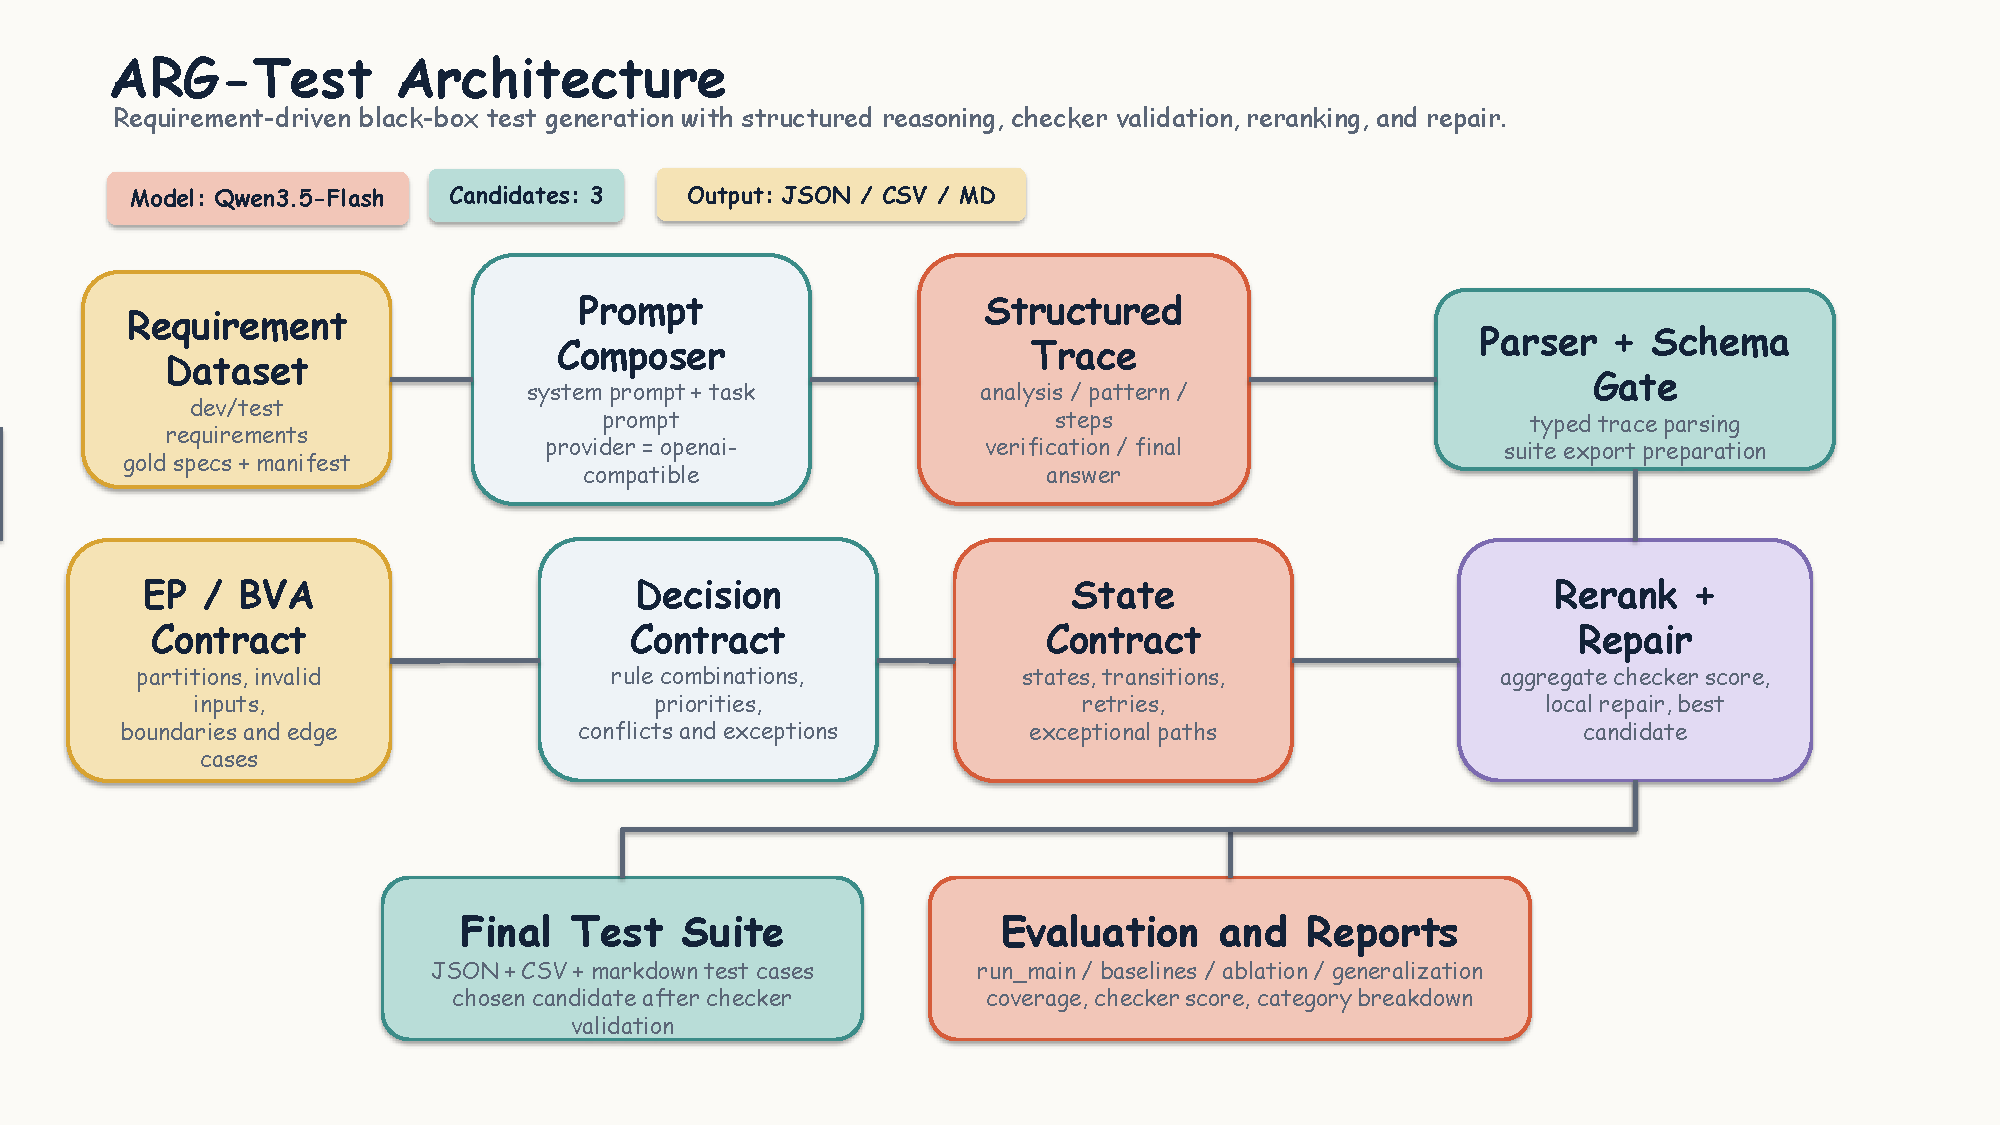
\includegraphics[width=\textwidth]{figures/arg_test_architecture_final.pdf}
\caption{The ARG-Test pipeline starts from requirement documents, produces multiple structured candidate traces, validates them with schema and technique-aware contracts, optionally repairs weak traces, attaches risk and state-model metadata, and exports final artifacts together with report-ready summaries.}
\label{fig:architecture}
\end{figure*}

Figure~\ref{fig:architecture} shows the main control flow. The design has five key modules: structured trace generation, parser/schema gating, technique-aware contract checking, candidate reranking plus repair, and evidence-oriented export. The final version adds two supporting modules that were not present in the earliest prototype: risk-aware prioritization and explicit state-model extraction.

\subsection{Structured Testing Trace}
The central representation is a five-section testing trace:
\begin{enumerate}[leftmargin=1.5em]
\item \texttt{Analysis}: entities, constraints, rules, fields, states, and exceptions extracted from the requirement.
\item \texttt{Pattern}: selected black-box testing techniques and the rationale for using them.
\item \texttt{Steps}: explicit derivation of partitions, boundaries, decision rules, or state transitions.
\item \texttt{Verification}: internal cross-checks against omissions or contradictions.
\item \texttt{FinalAnswer}: a normalized markdown table of final test cases with expected outputs and priorities.
\end{enumerate}

This structure matters because it converts hidden LLM reasoning into a checkable interface. If the model claims BVA, it must expose the relevant thresholds and neighboring cases. If it claims State Transition Testing, it must reveal states, triggers, legal transitions, and blocked transitions. The structured trace is therefore the backbone that enables the later deterministic checks.

\subsection{Parser, Contracts, and Candidate Control}
The parser converts raw model output into typed internal objects and acts as the first deterministic quality gate. It verifies whether the required sections exist, whether the final table is parseable, and whether required fields such as expected output and covered item are present. Once a trace passes this schema gate, ARG-Test applies one schema checker and four technique-aware checkers:
\begin{itemize}[leftmargin=1.5em]
\item EP checker: looks for representative valid and invalid partitions.
\item BVA checker: checks lower-boundary, on-boundary, and upper-boundary coverage obligations.
\item Decision checker: validates rule combinations and rule mapping depth.
\item State checker: validates states, legal transitions, illegal transitions, and exception paths.
\end{itemize}

Instead of trusting a single model sample, ARG-Test generates three candidates in the full setting and assigns them deterministic candidate-control profiles such as balanced coverage, boundary/rule emphasis, and negative/state stress. The system then reranks candidates according to checker outputs and duplicate penalties. If the best candidate remains weak, targeted repair adds the missing obligations while preserving already valid cases. This module works because it reduces the cost of stochastic model variance without discarding good partial reasoning.

\subsection{Risk-Aware Prioritization}
The final project adds a requirement-level risk model and case-level priority promotion. The risk score is computed from interpretable signals in the requirement text and parsed trace, including rule density, numeric constraints, selected techniques, business-impact keywords, strict rejection language, and workflow cues. The current implementation categorizes requirements into Low, Medium, or High risk and also records human-readable drivers such as ``7 explicit rule lines'' or ``decision-table logic.''

This module is needed because a final testing tool should not only generate cases; it should also explain where test effort should be concentrated. A requirement that mixes multiple rules, monetary impact, and strict rejection conditions should not be treated the same as a simple mandatory-field rule. In the final formal result, the average risk score on the frozen test split is \textbf{7.322} and \textbf{9 of 16} requirements are classified as High risk, which confirms that the held-out evaluation set contains many non-trivial scenarios rather than only easy toy examples.

\subsection{State-Model Extraction and Sequence Planning}
State Transition Testing in the final project is not limited to tagging a case as ``state related.'' ARG-Test now extracts explicit states, start states, legal transitions, illegal transitions, and coverage plans. When a requirement selects State Transition Testing, the pipeline builds a state model with two coverage goals: \textbf{All States} and \textbf{All Transitions}. Each goal is materialized as one or more executable sequence plans.

This module addresses a common weakness of free-form LLM outputs: they may mention a workflow but fail to enumerate the exact transition structure. By extracting states and transitions explicitly, the final project makes stateful requirements more auditable and aligns them with classical model-based testing expectations. This is one of the main reasons the workflow-state category performs strongly in the final evaluation.

\subsection{Input Interfaces and Reproducibility Controls}
The final version extends usability and reproducibility at the same time. Users can process a single requirement file, direct text input, or a CSV batch through the same CLI surface. In addition, runtime manifests now record provider, model, candidate count, API mode, seed, temperature, and top-\textit{p}. Seed-aware repeatability studies and replay from frozen raw generations are implemented as first-class experiment scripts rather than as informal notes. This is important because a final project must defend both how the tool is used and how its results are reconstructed.

\section{Implementation}
\subsection{Repository Modules}
\begin{table*}[t]
\centering
\small
\caption{Main implementation modules in the final ARG-Test repository.}
\label{tab:modules}
\begin{tabular}{p{0.18\textwidth} p{0.30\textwidth} p{0.40\textwidth}}
\toprule
\textbf{Module} & \textbf{Role} & \textbf{Main files} \\
\midrule
Prompt construction & Compose structured, baseline, and repair prompts & \texttt{prompts/}, \texttt{src/pipeline.py} \\
LLM client & Call mock or OpenAI-compatible providers with runtime metadata capture & \texttt{src/llm\_client.py}, \texttt{src/config.py} \\
Parser and schemas & Parse traces and test tables into typed objects & \texttt{src/parser.py}, \texttt{src/schemas.py} \\
Checker suite & Schema, EP, BVA, decision, and state validation & \texttt{src/checker/} \\
Reranking and repair & Select and patch the best candidate trace & \texttt{src/reranker.py}, \texttt{src/repair.py} \\
Risk scoring & Assess requirement risk and promote case priorities & \texttt{src/risk.py} \\
State modeling & Extract explicit state models and coverage plans & \texttt{src/state\_model.py} \\
Input loading & Read requirements from files, direct text, or CSV & \texttt{src/main.py}, \texttt{src/input\_loader.py} \\
Evaluation and export & Compute coverage metrics and save report artifacts & \texttt{src/evaluation/metrics.py}, \texttt{src/exporter.py} \\
Experiment scripts & Main, baseline, ablation, repeatability, replay, and validation workflows & \texttt{experiments/} \\
\bottomrule
\end{tabular}
\end{table*}

\subsection{Tool Configuration}
\begin{table}[h]
\centering
\small
\caption{Final tool configuration used for the canonical formal result.}
\label{tab:toolconfig}
\begin{tabular}{p{0.44\columnwidth} p{0.41\columnwidth}}
\toprule
\textbf{Item} & \textbf{Final setting} \\
\midrule
Input type & Natural-language requirement documents, direct text, CSV batches \\
Testing scope & AI-enhanced requirement-driven black-box dynamic testing \\
Supported techniques & EP, BVA, Decision Table Testing, State Transition Testing \\
Model & \texttt{qwen3.5-flash} \\
Provider interface & OpenAI-compatible endpoint \\
API mode for seeded study & \texttt{chat\_completions} \\
Candidate count & 3 \\
Repair & Enabled \\
Risk prioritization & Enabled \\
State-model extraction & Enabled when State Transition Testing is selected \\
Output formats & Markdown, JSON, CSV, manifest JSON \\
\bottomrule
\end{tabular}
\end{table}

The canonical formal result bundle under \texttt{.local\_runs/formal\_qwen\_novpn} is built from frozen live outputs and then enriched offline with the new final-project metadata such as risk scores, state models, and manifests. This design lets the final report reference a single stable result root without hiding how the upgraded evidence package was assembled.

\subsection{Exported Artifact Types}
For each processed requirement, ARG-Test exports raw generations, parsed traces, candidate-level metadata, checker logs, final test suites in Markdown/JSON/CSV, and per-requirement summaries. At the aggregate level, it exports formal report bundles for main comparison, baselines, ablation, category-level generalization, repeatability, and validation evidence. This artifact design directly supports the course requirement to submit prompts, model settings, generated outputs, and analysis.

\section{Experimental Setup}
\subsection{Requirement Dataset}
The dataset is an internally authored requirement collection centered on e-commerce and service-platform scenarios such as coupon rules, refund logic, pickup workflows, card validation, stateful payment authentication, and address-format constraints. We use a frozen \texttt{dev}/\texttt{test} split to separate prompt-checker tuning from final evaluation.

\begin{table}[h]
\centering
\small
\caption{Dataset distribution by split and requirement category.}
\label{tab:dataset}
\begin{tabular}{lrrrr}
\toprule
\textbf{Split} & \textbf{Business} & \textbf{Input} & \textbf{Workflow} & \textbf{Total} \\
 & \textbf{Rules} & \textbf{Validation} & \textbf{State} & \\
\midrule
Dev & 30 & 11 & 9 & 50 \\
Test & 7 & 4 & 5 & 16 \\
Total & 37 & 15 & 14 & 66 \\
\bottomrule
\end{tabular}
\end{table}

\subsection{Gold Specifications and Metrics}
Each requirement has a gold specification used for evaluation. Depending on the requirement type, the gold spec may contain valid partitions, invalid partitions, boundaries, decision rules, states, illegal transitions, and exception cases. We report three primary metrics:
\begin{itemize}[leftmargin=1.5em]
\item \texttt{checker\_score}: aggregate quality score from schema and technique-aware checks.
\item \texttt{overall\_coverage}: average coverage across \emph{applicable} dimensions only.
\item \texttt{test\_count}: number of final test cases in the exported suite.
\end{itemize}

We also track duplicate counts, category-level averages, risk metadata, and case-level diagnostics. A key design choice is that non-applicable dimensions are excluded rather than counted as automatic full marks; this prevents inflated scores on requirements that do not involve states or decision tables.

\subsection{Baselines and Ablation Protocol}
We compare ARG-Test against three baselines:
\begin{enumerate}[leftmargin=1.5em]
\item \textbf{Rule-based baseline}: deterministic heuristics for ranges, mandatory fields, and simple patterns.
\item \textbf{Plain LLM baseline}: direct prompting without structured trace constraints.
\item \textbf{Structured-no-checker baseline}: structured trace generation without checker-guided control or repair.
\end{enumerate}

These baselines answer complementary questions: whether AI helps relative to traditional automation, whether structured reasoning helps relative to plain prompting, and whether checker-guided control adds value beyond structure alone. The ablation in Section 6.4 therefore isolates checker-guided control by comparing the full pipeline against the structured-no-checker variant on the same frozen test split.

\subsection{Formal Result Source and Runtime Protocol}
The canonical formal report source is \texttt{.local\_runs/formal\_qwen\_novpn}. The corresponding manifests record provider, model, candidate count, repair setting, and the 16 frozen test IDs. The final report also references three auxiliary evidence sources:
\begin{itemize}[leftmargin=1.5em]
\item detailed executable evidence for \texttt{coupon\_discount\_engine},
\item non-functional validation summaries,
\item seeded repeatability and replay evidence.
\end{itemize}

This protocol is intentionally stronger than the middle-phase version because the final project must defend not only the main metric table but also how the reported bundle can be audited and reconstructed.

\section{Results}
\subsection{Overall Scorecard}
\begin{figure}[t]
\centering

\includegraphics[width=\columnwidth]{figures/final_result_scorecard.pdf}
\caption{Compact overview of the canonical formal result on the frozen 16-requirement test split.}
\label{fig:scorecard}
\end{figure}

The overall result is strong for a course final project. ARG-Test processes all \textbf{16 test requirements}, reaches an \textbf{average checker score of 0.959}, and maintains an \textbf{average overall coverage of 0.615}. No duplicate cases remain in the exported final suites. Moreover, \textbf{4 of 16} requirements are explicitly marked as repaired, which shows that the repair mechanism is used selectively rather than indiscriminately.

\subsection{Main Comparison Against Baselines}
\begin{figure}[t]
\centering

\includegraphics[width=\columnwidth]{figures/main_vs_baselines.pdf}
\caption{ARG-Test substantially outperforms traditional and weaker AI baselines on the frozen test split.}
\label{fig:mainvsbase}
\end{figure}

\begin{table*}[t]
\centering
\small
\caption{Main comparison on the frozen test split.}
\label{tab:maincomparison}
\begin{tabular}{lccc}
\toprule
\textbf{Method} & \textbf{Avg checker score} & \textbf{Avg overall coverage} & \textbf{Avg test count} \\
\midrule
Rule-based & 0.753 & 0.147 & 4.125 \\
Plain LLM & 0.844 & 0.030 & 7.250 \\
Structured No Checker & 0.841 & 0.538 & 6.312 \\
\textbf{ARG-Test Full Pipeline} & \textbf{0.959} & \textbf{0.615} & \textbf{7.312} \\
\bottomrule
\end{tabular}
\end{table*}

Table~\ref{tab:maincomparison} supports three conclusions. First, the full pipeline is clearly better than the traditional non-AI baseline. Second, plain LLM prompting produces many fluent cases but almost no useful coverage, which confirms that direct prompting alone is not enough. Third, the full pipeline also improves over the standardized structured-no-checker baseline, which means that parser-plus-checker control matters in practice and is not just decorative engineering.

The pairwise win counts are also favorable. The full pipeline beats the rule-based baseline on both checker score and coverage for \textbf{16/16} requirements, and it does the same against the plain-LLM baseline for \textbf{16/16} requirements. Against the standardized structured-no-checker baseline, it improves checker score for \textbf{11/16} requirements and coverage for \textbf{11/16} requirements, while also improving the aggregate averages from \textbf{0.841} to \textbf{0.959} in checker score and from \textbf{0.538} to \textbf{0.615} in coverage.

\subsection{Generalization Across Requirement Categories}
\begin{figure}[t]
\centering

\includegraphics[width=\columnwidth]{figures/generalization_by_category.pdf}
\caption{The full pipeline remains effective across business-rule, input-validation, and workflow-state requirements.}
\label{fig:generalization}
\end{figure}

\begin{table}[h]
\centering
\small
\caption{Category-level generalization and risk profile on the frozen test split.}
\label{tab:generalization}
\begin{tabular}{lcccc}
\toprule
\textbf{Category} & \textbf{Count} & \textbf{Avg score} & \textbf{Avg coverage} & \textbf{Avg risk} \\
\midrule
Business Rules & 7 & 0.957 & 0.577 & 7.729 \\
Input Validation & 4 & 0.950 & 0.579 & 7.250 \\
Workflow State & 5 & 0.970 & 0.697 & 6.810 \\
\bottomrule
\end{tabular}
\end{table}

These results show that the system does not only work on one convenient category. Workflow-state requirements are the strongest category, with an average checker score of \textbf{0.970} and average coverage of \textbf{0.697}. This is consistent with the fact that explicit states and transition triggers are often easier to recover from text than open-ended address or formatting constraints. At the same time, both business-rule and input-validation requirements remain solid, with coverage around \textbf{0.58} and average scores near \textbf{0.95}. The category-level risk averages also show that the final dataset is not biased toward only simple cases.

\subsection{Ablation}
\begin{figure}[t]
\centering

\includegraphics[width=\columnwidth]{figures/ablation_gain.pdf}
\caption{Ablation aligned with the frozen test split: checker-guided control improves quality over the structured-no-checker variant while keeping test-suite breadth competitive.}
\label{fig:ablation}
\end{figure}

The ablation result is instructive even without a second table because it can be read directly against Table~\ref{tab:maincomparison}. The structured-no-checker variant reaches \textbf{0.841} checker score, \textbf{0.538} overall coverage, and \textbf{6.312} test cases on average, whereas the full pipeline reaches \textbf{0.959} checker score, \textbf{0.615} coverage, and \textbf{7.312} test cases. The message is therefore straightforward: checker-guided selection and repair do not merely polish presentation; they materially improve checker-aligned quality and also improve practical coverage. The checker-score gain from \textbf{0.841} to \textbf{0.959} is large, and the coverage gain from \textbf{0.538} to \textbf{0.615} confirms that contract-guided control improves obligation completeness rather than only pruning cases.

\subsection{Representative Case Breadth}
\begin{figure*}[t]
\centering

\includegraphics[width=\textwidth]{figures/case_study_snapshots.pdf}
\caption{Representative outputs from business-rule, input-validation, and workflow-state requirements.}
\label{fig:casestudy}
\end{figure*}

Figure~\ref{fig:casestudy} illustrates category breadth using business-rule, input-validation, and workflow-state examples. This matters because the strongest signal of practical usefulness is not a single good requirement but the ability to handle diverse requirement structures with the same pipeline.

\section{Detailed Module Execution and Usefulness}
\subsection{Why \texttt{coupon\_discount\_engine} Was Chosen}
The final project requires at least one detailed module-level design and execution study. We selected \texttt{coupon\_discount\_engine} because it sits at the intersection of rule combinations, numeric boundaries, invalid-input handling, and business-critical money logic. It is also a High-risk requirement in the formal result, with risk score \textbf{8.85}, checker score \textbf{0.95}, and overall coverage \textbf{0.683}. This makes it a strong anchor for both black-box and white-box evidence.

\subsection{Executable Black-Box and White-Box Evidence}
\begin{table}[h]
\centering
\small
\caption{Detailed execution evidence for \texttt{coupon\_discount\_engine}.}
\label{tab:detailedmodule}
\begin{tabular}{p{0.50\columnwidth} p{0.27\columnwidth}}
\toprule
\textbf{Item} & \textbf{Observed result} \\
\midrule
Black-box and white-box executable tests & 15 passed \\
Repository regression suite at report-preparation time & 27 passed \\
Statement coverage on the reference module & 100\% \\
Branch coverage on the reference module & 100\% \\
Mutation demonstration & 4 mutants killed out of 4 \\
Mutation kill rate & 1.0 \\
\bottomrule
\end{tabular}
\end{table}

Table~\ref{tab:detailedmodule} shows that the detailed case study is not just a narrative walkthrough. It is backed by executable tests, coverage reports, and defect-seeded usefulness evidence. The black-box portion targets threshold cases, invalid coupon combinations, and rule-priority logic. The white-box portion targets branches in the reference implementation. Together they provide the concrete execution anchor that the middle-phase system still lacked.

\subsection{Mutation-Based Usefulness Demonstration}
The final project also includes a defect-seeded usefulness demonstration. We created four mutants for the reference implementation: one that incorrectly allows multiple coupons, one that rejects \texttt{SAVE10} exactly at the subtotal-50 boundary, one that ignores the \texttt{SAVE20} sale-item restriction, and one that rejects \texttt{FREESHIP} exactly at the subtotal-30 boundary. The curated executable suite kills \textbf{all four mutants}. This result is important because it shows that the generated or derived tests are not only structurally plausible; they are also strong enough to detect realistic seeded faults.

\section{Non-Functional and Practical Validation}
\begin{table*}[t]
\centering
\small
\caption{Non-functional validation summary for the final system.}
\label{tab:nfr}
\begin{tabular}{p{0.16\textwidth} p{0.72\textwidth}}
\toprule
\textbf{Dimension} & \textbf{Observed evidence} \\
\midrule
Performance & On a five-requirement mock sample, average processing time is about 0.005 seconds per requirement, which is sufficient for local validation workflows. \\
Usability & The CLI supports \texttt{batch}, \texttt{batch-csv}, \texttt{run}, \texttt{run-text}, and \texttt{state-model}; the repository provides a README quick start, a formal workflow script, and JSON/CSV/Markdown outputs. \\
Security & No secret leak is found in generated or report artifacts, and manifests record provider metadata without exposing API keys. \\
Maintainability & The repository is organized into modular \texttt{src/}, \texttt{experiments/}, \texttt{tests/}, and \texttt{report\_assets/} layers, and the final regression suite passes at report-preparation time. \\
Runtime isolation & Result bundles are separated by output roots, which prevents one experiment from silently overwriting another. \\
\bottomrule
\end{tabular}
\end{table*}

This non-functional validation is useful for two reasons. First, it demonstrates that the project is usable as a tool rather than only as a one-time experiment. Second, it shows that engineering quality was considered explicitly in the final phase. The final project is still a student system, so the NFR analysis is lightweight rather than industrial-grade, but it is concrete and evidence-backed.

\section{Reproducibility and Stability}
\subsection{Seeded Repeatability and Replay}
\begin{table*}[t]
\centering
\small
\caption{Reproducibility and stability evidence in the final project.}
\label{tab:repro}
\begin{tabular}{p{0.24\textwidth} p{0.19\textwidth} p{0.45\textwidth}}
\toprule
\textbf{Evidence type} & \textbf{Observed result} & \textbf{Interpretation} \\
\midrule
Mock 3-seed repeatability & 16/16 stable; score delta 0.0; coverage delta 0.0 & The repository-level deterministic chain, manifests, and repeatability aggregator are wired correctly. \\
Live multi-seed sample & 1/5 stable; average score 0.91; average coverage 0.576 & Live seeded experiments are supported, but the current upstream endpoint still shows residual nondeterminism. \\
Live same-seed sample & 0/3 stable under a fixed seed schedule & The current provider does not guarantee strict deterministic replay even when the same seed is reused. \\
Archive-grade replay & Frozen raw generations can be replayed offline into a new result bundle & Submission-level reproducibility is achieved through saved generations plus offline replay rather than by assuming provider determinism. \\
\bottomrule
\end{tabular}
\end{table*}

Figure~\ref{fig:repro} complements Table~\ref{tab:repro} by presenting the engineering conclusion first and the raw repeatability evidence second. The intended message is positive but precise: ARG-Test already achieves strong pipeline-level reproducibility, and the remaining live variance is explicitly contained by frozen generations plus replay.

\begin{figure*}[t]
\centering
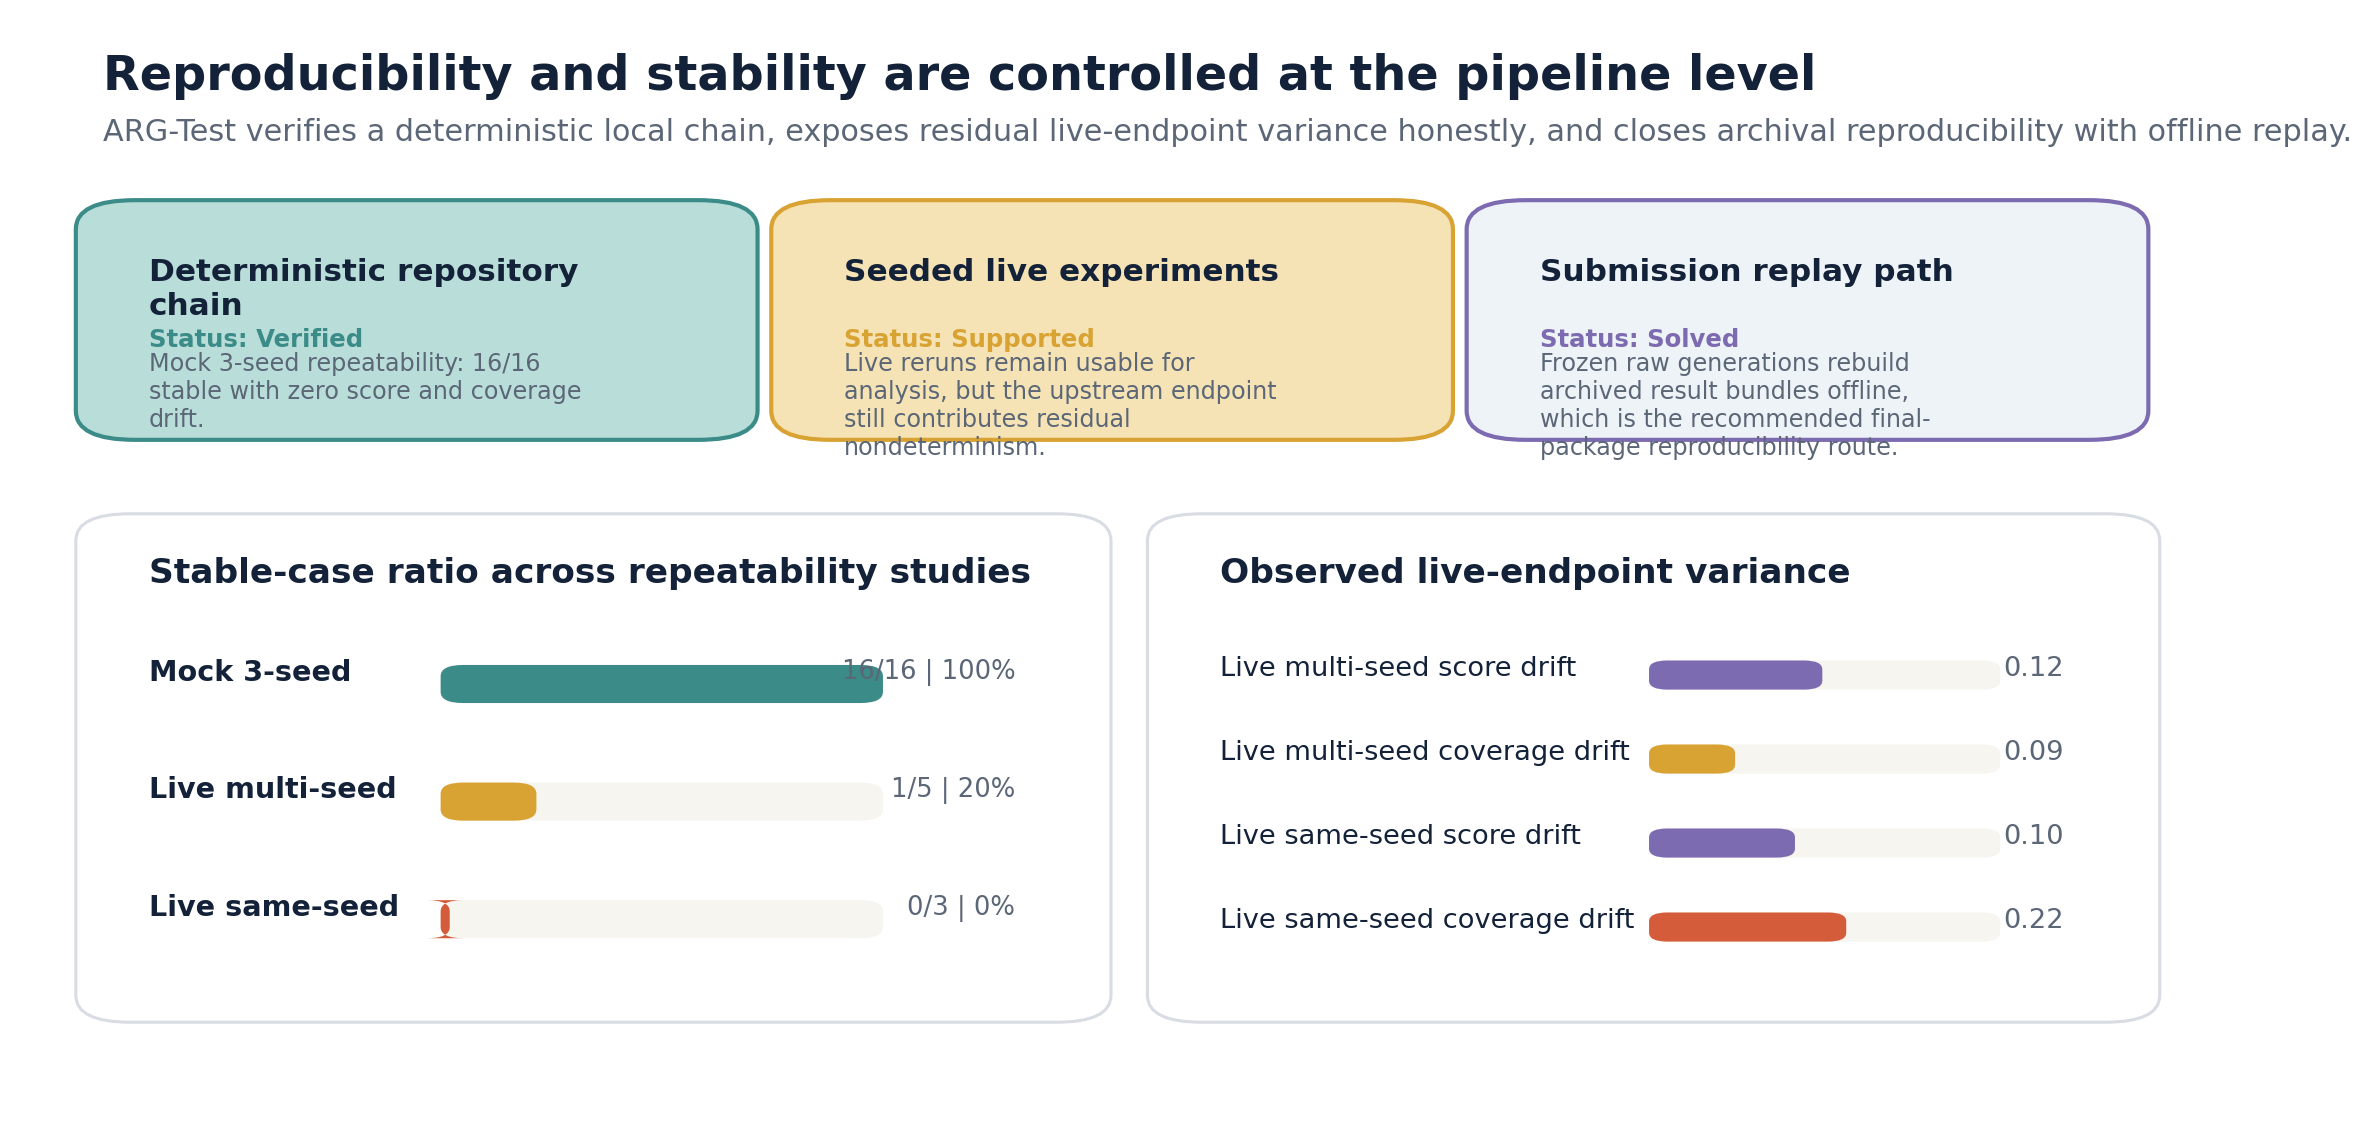
\includegraphics[width=0.94\textwidth]{figures/reproducibility_stability_overview.png}
\caption{Formal reproducibility and stability overview. The figure highlights three takeaways: the repository chain is deterministic under seeded mock control, live seeded studies remain usable but expose some provider variance, and archive-grade replay provides the final submission-level reproducibility guarantee.}
\label{fig:repro}
\end{figure*}

This section should be read in two layers. At the \emph{pipeline layer}, the result is already strong: seeded mock experiments show that manifests, candidate control, parsing, checking, reranking, repair, and reporting form a deterministic local chain. At the \emph{provider layer}, the current live endpoint still introduces some residual variance, so the final report deliberately avoids overclaiming strict live determinism.

\subsection{Why This Still Strengthens the Final Project}
This distinction still strengthens the project rather than weakening it. A mature final submission should separate what it can control locally from what belongs to the upstream model service. ARG-Test does this explicitly. It uses seeded experimentation, multi-candidate selection, and targeted repair to stabilize the local workflow, and it uses frozen generations plus offline replay to guarantee submission-level reproducibility for the archived package. That is a more defensible engineering claim than pretending the provider itself is perfectly deterministic.

\section{Comparison with a Traditional Non-AI Technique}
\begin{table*}[t]
\centering
\small
\caption{Traditional non-AI rule-based baseline versus ARG-Test.}
\label{tab:nonai}
\begin{tabular}{p{0.18\textwidth} p{0.31\textwidth} p{0.31\textwidth}}
\toprule
\textbf{Aspect} & \textbf{Traditional rule-based baseline} & \textbf{ARG-Test full pipeline} \\
\midrule
Core mechanism & Deterministic pattern rules & LLM generation plus parser, checker, reranking, repair, and risk-aware enrichment \\
Language flexibility & Weak on implicit logic and mixed constraints & Strong on realistic natural-language interpretation \\
Auditability & High only for the rules it already knows & High due to structured traces, checker logs, manifests, and exported summaries \\
Cost & Very low & Moderate API cost and engineering complexity \\
Variance & Deterministic & Stochastic at provider level but controlled and replayable at pipeline level \\
Coverage on frozen test split & 0.147 & 0.615 \\
Best use case & Simple mandatory-field or range heuristics & Mixed business-rule, validation, and workflow requirements \\
\bottomrule
\end{tabular}
\end{table*}

The comparison in Table~\ref{tab:nonai} answers the course requirement to compare an AI-enhanced technique against a traditional non-AI approach. The rule-based baseline is cheap and deterministic, which is attractive, but it cannot recover enough structure from realistic natural-language requirements. ARG-Test is more expensive and more complex, yet it is dramatically stronger in coverage and artifact richness. For this final project, that trade-off is justified.

\section{Discussion and Limitations}
\subsection{Why the Final System Works}
The final system works because it avoids asking the model to solve the entire testing problem in one opaque step. The structured trace exposes the reasoning, the contract checkers turn testing theory into deterministic obligations, and reranking plus repair reduce the effect of single-sample errors. Risk scoring and state-model extraction then make the result more actionable and better aligned with a practical testing workflow. In short, the project succeeds because it combines LLM flexibility with deterministic control layers.

\subsection{Remaining Limitations}
The final report should still state its limitations explicitly.
\begin{enumerate}[leftmargin=1.5em]
\item The project focuses on the requirement-driven branch rather than the codebase-driven branch, so conclusions apply to requirement-based black-box test design.
\item The frozen test split has 16 requirements, which is sufficient for a course final project but not a large benchmark study.
\item Coverage metrics depend on authored gold specifications, so evaluation quality still depends on the quality of the gold definitions.
\item The detailed executable evidence is strong for the chosen module, but the full 16-requirement benchmark is still evaluated mainly at the test-design level rather than by executing every generated suite against a real implementation.
\item Provider-level live determinism is limited, so strong reproducibility claims must rely on frozen generations and replay instead of on the provider alone.
\end{enumerate}

\subsection{Threats to Validity and Practical Interpretation}
These limitations define scope rather than failure. Within that scope, the project is already strong: it is auditable, reproducible at the submission level, substantially stronger than traditional and prompt-only baselines, and supported by concrete executable evidence. The correct final interpretation is therefore not that the system is perfect, but that it is a high-quality course project with honest boundaries and unusually complete engineering support.

\section{Conclusion}
This report presented ARG-Test, a requirement-driven AI-enhanced testing tool that transforms natural-language requirements into auditable black-box test suites. The key idea is simple but effective: do not trust a free-form model answer; instead, require a structured testing trace, validate it against testing-theory contracts, control variance with reranking and repair, and preserve enough metadata to audit and reproduce the result later.

The strongest evidence is empirical. On the frozen 16-requirement test split, ARG-Test reaches an average checker score of 0.959 and average overall coverage of 0.615, clearly outperforming rule-based automation, plain LLM prompting, and weaker structured variants. The project is further strengthened by detailed executable evidence for \texttt{coupon\_discount\_engine}, mutation-based usefulness demonstration, non-functional validation, and archive-grade replay support.

A current limitation is scope rather than collapse: the project focuses on requirement-driven black-box testing and still depends on a non-deterministic live provider. Extending the same audited pipeline to broader executable benchmarks or stronger provider-level determinism would be a natural next step. Even with that limitation, ARG-Test already satisfies the final-project requirements at a level significantly above a minimal submission and provides a defendable end-to-end artifact package.

\clearpage
\onecolumn
\appendix
\section{Prompt Artifacts}
\subsection{System Prompt Snippet}
\begin{verbatim}
You are a software testing expert.
Given a natural-language requirement, produce a structured black-box
testing trace with exactly five sections:
Analysis, Pattern, Steps, Verification, FinalAnswer.
\end{verbatim}

\subsection{Generation Prompt Skeleton}
\begin{verbatim}
Requirement:
{{REQUIREMENT_TEXT}}

Task:
Generate black-box test cases using a structured testing trace.

Output format:
Analysis:
...
Pattern:
...
Steps:
1. ...
Verification:
- Verified against Step 1 and Step 2.
FinalAnswer:
| Test ID | Technique | Requirement Target |
| Preconditions | Input | Expected Output |
| Covered Item | Priority | Checker Status |
\end{verbatim}

\subsection{Repair Prompt Skeleton}
\begin{verbatim}
The previous structured testing trace failed the contract checker.

Requirement:
{{REQUIREMENT_TEXT}}

Previous trace:
{{RAW_TRACE}}

Diagnostics:
{{DIAGNOSTICS}}

Revise only the necessary parts.
Keep the five-section structure unchanged.
Preserve correct test cases.
Remove duplicate or contradictory test cases.
Return the full corrected trace.
\end{verbatim}

\section{Representative Commands}
\subsection{Formal Main Workflow}
\begin{verbatim}
powershell -ExecutionPolicy Bypass
  -File experiments/run_formal_workflow.ps1
  -Provider openai
  -Model qwen3.5-flash
  -OutputRoot .local_runs/formal_qwen_novpn
\end{verbatim}

\subsection{Direct Text and CSV Entry Points}
\begin{verbatim}
python -m src.main run-text --text "..." --provider mock
python -m src.main batch-csv --input requirements.csv --provider mock
\end{verbatim}

\subsection{Repeatability and Replay}
\begin{verbatim}
python experiments/run_repeatability.py --split test --provider mock
python experiments/replay_seeded_runtime.py
  --source-root .local_runs/repro_multi_seed_mock
  --output-root .local_runs/replay_mock_smoke
\end{verbatim}

\subsection{Detailed Module Execution}
\begin{verbatim}
python -m pytest tests\test_coupon_discount_engine_blackbox.py
python -m pytest tests\test_coupon_discount_engine_whitebox.py
python -m coverage run --branch -m pytest tests -q
\end{verbatim}

\section{Representative Output Example}
The following excerpt shows the normalized output style used by ARG-Test for workflow-state requirements.

\begin{table}[h]
\centering
\scriptsize
\caption{Representative generated test cases for a workflow-state requirement.}
\label{tab:outputexample}
\begin{tabular}{p{0.08\textwidth} p{0.10\textwidth} p{0.10\textwidth} p{0.11\textwidth} p{0.12\textwidth} p{0.16\textwidth} p{0.11\textwidth}}
\toprule
\textbf{Test ID} & \textbf{Technique} & \textbf{Requirement Target} & \textbf{Preconditions} & \textbf{Input} & \textbf{Expected Output} & \textbf{Covered Item} \\
\midrule
T01 & State Transition & Req 2, 3 & None & Card flagged for 3DS & Status: AUTH\_REQUIRED & Initial flow start \\
T02 & State Transition & Req 3 & Status: AUTH\_REQUIRED & Valid 3DS token & Status: AUTHENTICATED & Successful auth \\
T03 & State Transition & Req 6 & Status: FAILED & Third retry attempt & Error: MAX\_RETRY\_EXCEEDED & Retry limit enforcement \\
T04 & State Transition & Req 7 & Status: INITIATED & POST /Capture & Error: MISSING\_AUTH & Illegal transition blocking \\
T05 & State Transition & Req 5 & Status: AUTH\_REQUIRED & Provider timeout event & Status: PENDING\_REVIEW & Timeout handling \\
\bottomrule
\end{tabular}
\end{table}

\section*{References}
\noindent [1] Course Staff. \emph{Assignment 2 Final Project: AI-Enhanced Software Testing}. 2026.\\
\noindent [2] Glenford J. Myers, Corey Sandler, and Tom Badgett. \emph{The Art of Software Testing}. Wiley, third edition, 2011.\\
\noindent [3] Paul C. Jorgensen. \emph{Software Testing: A Craftsman's Approach}. CRC Press, fourth edition, 2013.\\
\noindent [4] Course-provided reference paper. \emph{Structured reasoning and verification reference paper} (\texttt{kr-paper324.pdf}). 2026.\\
\noindent [5] Qwen / OpenAI-compatible API documentation used during the project workflow. 2026.

\end{document}
